\documentclass[a2paper, 12pt]{article}
\usepackage[font={huge, bf}]{caption}
\usepackage{fontspec}
\setmainfont{Arial}
\usepackage{subcaption}
\usepackage{graphicx}
\usepackage{tikz}
\usepackage{tikzsymbols}
\usetikzlibrary{calc,patterns,shapes.geometric}
\usepackage{float}
\usepackage{pdflscape}
\usepackage{geometry}
\geometry{landscape, margin=2cm}
\captionsetup[subfigure]{justification=justified,singlelinecheck=false}
\pagestyle{empty}

\def\centerarc[#1](#2)(#3:#4:#5){\draw[#1] ($(#2)+({#5*cos(#3)},{#5*sin(#3)})$) arc (#3:#4:#5);}

\begin{document}
	\vspace*{\fill}
	\begin{figure}[!htbp]
		\centering
		\begin{subfigure}[b]{0.48\textwidth}
			\caption{Figure 1}
			\centering
			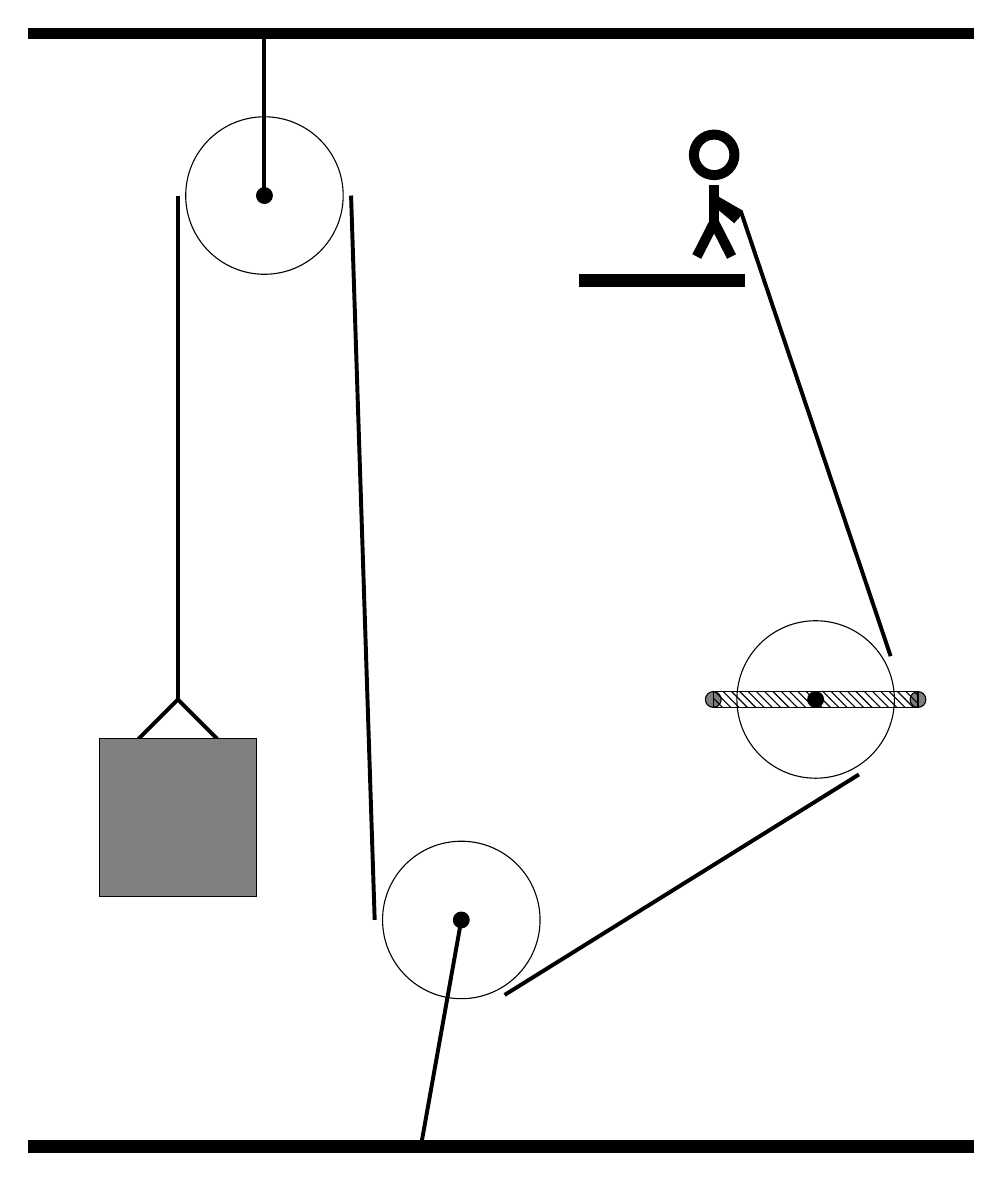
\begin{tikzpicture}
				\draw[fill=black] (-2, 14) rectangle (10, 14.125);
				
				\draw (1, 12) circle (1);
				\draw[fill=black] (1, 12) circle (0.1);
				\draw[line width=0.5mm] (1, 14) -- (1, 12);
				
				\draw (3.5, 2.8) circle (1);
				\draw[fill=black] (3.5, 2.8) circle (0.1);
				\draw[line width=0.5mm] (3.5, 2.8) -- (3.0, 0);
				
				\draw[fill=white](8, 5.6) circle (1);
				\draw[fill=black] (8, 5.6) circle (0.1);
				\draw[fill=black!50] (9.3, 5.6) circle (0.1);
				\draw[fill=black!50] (6.7, 5.6) circle (0.1);
				\draw[pattern=north west lines, pattern color=black] (6.7, 5.7) rectangle (9.3, 5.5);
				
				\draw[line width=0.5mm](-0.6, 5.1) --  (-0.1, 5.6) -- (0.4, 5.1);
				\draw[fill=black!50] (-1.1, 5.1) rectangle (0.9, 3.1);
				
				\draw[line width=0.5mm](-0.1, 12) -- (-0.1, 5.6);
				\centerarc[line width=0.5mm](1, 12)(180:0:1.1)
				\draw[line width=0.5mm](2.1, 12) -- (2.4, 2.8);
				\centerarc[line width=0.5mm](3.5, 2.8)(180:300:1.1);
				\draw[line width=0.5mm](4.05, 1.8474) -- (8.55, 4.6474);
				\centerarc[line width=0.5mm](8, 5.6)(300:390:1.1);
				\draw[line width=0.5mm](8.9526, 6.15) -- (7.05, 11.8);
				
				\node at (6.75, 12) {\scriptsize \Strichmaxerl[10][-220][-30]};
				\draw[fill=black] (5, 11) rectangle (7.1, 10.85);
				
				\draw[fill=black] (-2, 0) rectangle (10, -0.15);
			\end{tikzpicture}
		\end{subfigure}
		\hfill
		\begin{subfigure}[b]{0.48\textwidth}
			\caption{Figure 2}
			\centering
			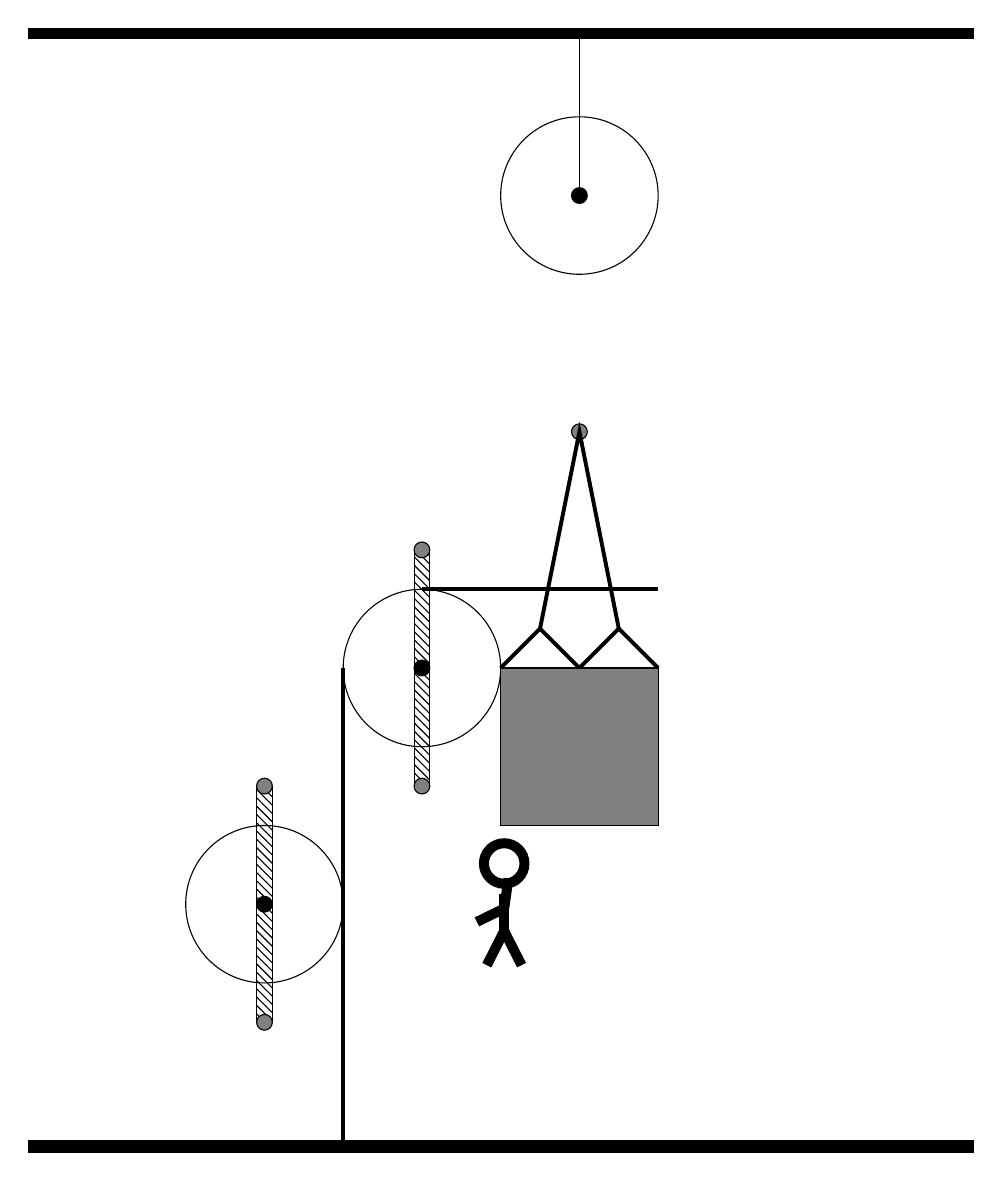
\begin{tikzpicture}
				\draw[fill=black] (-2, 14) rectangle (10, 14.125);
				
				\draw (1,3) circle (1);
				\draw[fill=black] (1,3) circle (0.1);
				\draw[pattern=north west lines, pattern color=black] (0.9,4.5) rectangle (1.1,1.5);
				\draw[fill=black!50] (1,4.5) circle (0.1);
				\draw[fill=black!50] (1,1.5) circle (0.1);
				
				\draw (5,12) circle (1);
				\draw[fill=black] (5,12) circle (0.1);
				\draw (5,14.0) -- (5,12);
				
				\draw (3,6) circle (1);
				\draw[fill=black] (3,6) circle (0.1);
				\draw[pattern=north west lines, pattern color=black] (2.9,7.5) rectangle (3.1,4.5);
				\draw[fill=black!50] (3,7.5) circle (0.1);
				\draw[fill=black!50] (3,4.5) circle (0.1);
				
				\draw[fill=black!50] (5,9) circle (0.1);
				\draw[line width=0.5mm](4.5,6.5) -- (5,9) --  (5.5,6.5);
				\draw[line width=0.5mm](4,6) --  (4.5,6.5) -- (5,6) -- (5.5,6.5) -- (6,6);
				\draw[fill=black!50] (4, 6) rectangle (6, 4);
				
				\draw[line width = 0.5mm] (3,7) -- (6,7);
				\centerarc[line width = 0.5mm](3,6)(90:180:1);
				\draw[line width = 0.5mm] (2,6) -- (2,0);
				\centerarc[line width = 0.5mm](3,0)(180:360:1);
				
				\node at (4, 3) {\scriptsize \Strichmaxerl[10][-98][-154]};
				
				\draw[fill=black] (-2, 0) rectangle (10, -0.15);
			\end{tikzpicture}
		\end{subfigure}
	\end{figure}
		\vspace*{\fill}
\end{document}